% ============================================================================
%  PRL Article: Modeling Two-Dimensional Supersonic Marshak Waves
%  Uses revtex4-2 (APS journal style)
% ============================================================================
\documentclass[prl, twocolumn, superscriptaddress, amsmath, amssymb, reprint]{revtex4-2}

\usepackage{graphicx}
\usepackage{amsmath}
\usepackage{amssymb}
\usepackage{bm}
\usepackage{hyperref}
\usepackage{xcolor}

\graphicspath{{figures/}}

\begin{document}

% ----------------------------------------------------------------------------
%  Title
% ----------------------------------------------------------------------------
\title{Semi-Analytic Two-Dimensional Model for Supersonic Marshak Waves in Cylindrical Geometry}

\author{Yuval Kochavi}
\affiliation{Racah Institute of Physics, The Hebrew University of Jerusalem, Jerusalem 91904, Israel}

\author{Tal Ramot}
\affiliation{Racah Institute of Physics, The Hebrew University of Jerusalem, Jerusalem 91904, Israel}

\author{Tal Balakirski}
\affiliation{Racah Institute of Physics, The Hebrew University of Jerusalem, Jerusalem 91904, Israel}

\author{Shay I.~Heizler}
\affiliation{Racah Institute of Physics, The Hebrew University of Jerusalem, Jerusalem 91904, Israel}

\date{\today}

% ----------------------------------------------------------------------------
%  Abstract
% ----------------------------------------------------------------------------
\begin{abstract}
We present a semi-analytic two-dimensional model for supersonic Marshak waves propagating through low-density foams confined in cylindrical tubes.
Starting from the one-dimensional Hammer--Rosen (HR) diffusion solution, we systematically incorporate the Marshak boundary condition, energy loss to tube walls, inward wall ablation with foam densification, and an effective mean free path correction for the wall-collision transport regime.
The resulting ``1.5D'' model accurately reproduces the longitudinal heat front position across seven independent experiments spanning diverse foam materials, densities, and drive temperatures.
We then extend the model to two dimensions by coupling the 1.5D longitudinal solution with a Bessel-function radial mode derived from the cylindrical diffusion eigenvalue problem, using a dynamically computed wall albedo.
The full 2D model captures the front curvature, the complete temperature distribution, and the spatial profile of the emerging radiation flux.
Comparisons with 2D diffusion simulations and experimental curvature measurements for gold- and copper-coated tubes demonstrate quantitative agreement, providing a unified, physically transparent framework for understanding radiation-driven heat waves in confined geometries.
\end{abstract}

\maketitle

% ============================================================================
%  I. INTRODUCTION
% ============================================================================
\section{Introduction}

Supersonic radiation-driven heat waves, known as Marshak waves~\cite{Marshak1958, Zel'dovich1967}, are central to inertial confinement fusion (ICF) and high-energy-density physics (HEDP)~\cite{Lindl2004}.
In a typical experiment, a hohlraum converts laser energy into thermal x-rays that drive a supersonic heat front into a low-density foam sample~\cite{Back2000PRL, Back2000POP, Moore2015}.
Because the wave speed exceeds the sound speed, the material ahead of the front remains unperturbed, and the problem reduces to nonlinear radiation diffusion.

Despite decades of study, quantitative modeling of these experiments has relied heavily on expensive numerical simulations---Implicit Monte Carlo (IMC) and deterministic transport codes---while analytic models remained limited to one dimension~\cite{Hammer2003, Shussman2015, Henyey1955}.
The one-dimensional (1D) Hammer--Rosen (HR) model~\cite{Hammer2003} provides a useful baseline but overestimates the front position by a factor of $\sim 2$ when compared to experiments~\cite{Back2000POP}, because it neglects boundary condition corrections and all two-dimensional effects arising from the cylindrical tube geometry.

In this Letter, we develop a semi-analytic model that bridges the gap between 1D theory and full numerical simulation.
We first construct a ``1.5D'' model by augmenting the HR solution with four physically motivated corrections, then extend it to a full 2D model that captures the radial curvature of the heat front.
The model is validated against seven independent experiments and 2D diffusion simulations across multiple wall materials.

% ============================================================================
%  II. GOVERNING EQUATIONS
% ============================================================================
\section{Governing Equations}

The radiative transfer equation (RTE) for a scattering-free medium reads
\begin{equation}\label{eq:RTE}
    \frac{1}{c}\frac{\partial I}{\partial t}+\hat{\Omega}\cdot\nabla I = \sigma_a\!\left(B(T_m) - I\right),
\end{equation}
where $I(\hat{\Omega},\vec{r},t)$ is the specific intensity, $\sigma_a$ is the absorption coefficient, and $B(T_m)$ is the Planck function at the material temperature $T_m$.
Coupling to the material energy equation,
\begin{equation}\label{eq:material_energy}
    \frac{C_v}{c}\frac{\partial T_m}{\partial t} = \sigma_a\!\left(\frac{1}{c}\int_{4\pi} I\,d\hat{\Omega} - aT_m^4\right),
\end{equation}
and applying the diffusion approximation yields the gray coupled system
\begin{align}
    \frac{\partial E}{\partial t} - \nabla\!\cdot\!\left(\frac{c}{3\sigma}\nabla E\right) &= c\sigma(U - E),\label{eq:gray_rad}\\
    \frac{\partial e}{\partial t} &= c\sigma(E - U),\label{eq:gray_mat}
\end{align}
with radiation energy density $E = aT_R^4$, material energy density $U = aT_m^4$, and specific internal energy $e = fT_m^\beta\rho^{-\mu}$.

In the supersonic regime, assuming complete thermodynamic equilibrium ($T_R = T_m \equiv T$) and that the material energy dominates over the radiation energy ($\rho f T^\beta \rho^{-\mu} \gg aT^4$, valid for $T \lesssim 3$\,keV), Eqs.~(\ref{eq:gray_rad})--(\ref{eq:gray_mat}) reduce to a single nonlinear diffusion equation:
\begin{equation}\label{eq:diffusion}
    f\rho^{-\mu}\frac{\partial T^\beta}{\partial t} = \nabla\!\cdot\!\left(\frac{c}{3\sigma}\nabla(aT^4)\right).
\end{equation}
The material properties are described by power laws:
\begin{equation}\label{eq:power_laws}
    e = fT^\beta\rho^{-\mu}, \qquad \kappa^{-1} = gT^\alpha\rho^{-\lambda},
\end{equation}
where $f,\beta,\mu,g,\alpha,\lambda$ are material-dependent parameters.
The diffusion coefficient $D = c/(3\rho\kappa)$ is strongly nonlinear in temperature, making Eq.~(\ref{eq:diffusion}) analytically intractable in general.

% ============================================================================
%  III. THE 1.5D MODEL
% ============================================================================
\section{The 1.5D Model}

\subsection{Baseline: Hammer--Rosen solution}

Hammer and Rosen~\cite{Hammer2003} solved Eq.~(\ref{eq:diffusion}) in one dimension using perturbation theory.
The heat front position is given by
\begin{equation}\label{eq:HR}
    x_F^2(t) = \frac{2+\varepsilon}{1-\varepsilon}\,C\,H^{-\varepsilon}(t)\int_0^t H(t')\,dt',
\end{equation}
where $H(t) = T_s^{4+\alpha}(t)$, $\varepsilon = \beta/(4+\alpha)$, and
\begin{equation}\label{eq:C_coeff}
    C = \frac{16\,g\,\sigma_{\mathrm{SB}}}{3f(4+\alpha)}\,\rho^{2-\mu-\lambda}.
\end{equation}
Here $T_s$ is the surface temperature at $x = 0$, which HR set equal to the hohlraum drive temperature $T_D$.

\begin{figure}[t]
    \centering
    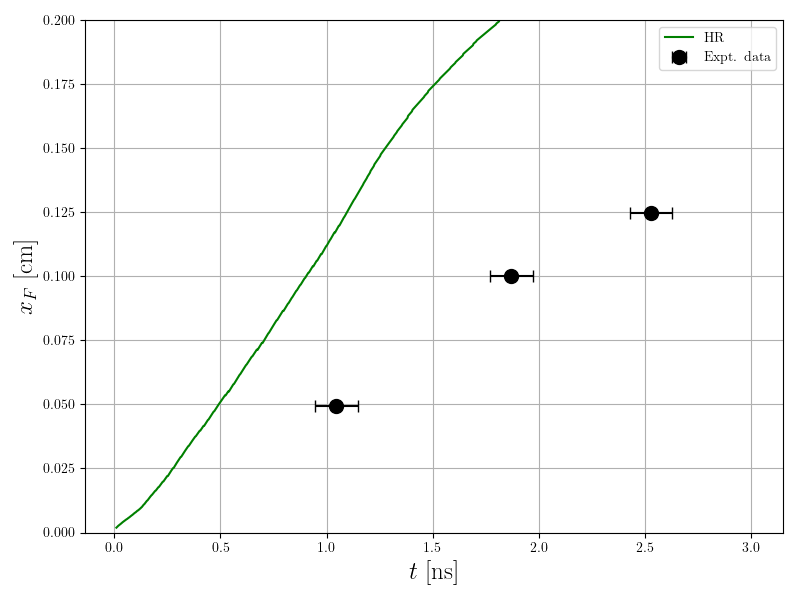
\includegraphics[width=\columnwidth]{figures/HR.png}
    \caption{Heat front position from the HR 1D model (dashed) compared to the experimental data of Back \textit{et al.}~\cite{Back2000POP}. The HR model overestimates the front position by approximately a factor of~2.}
    \label{fig:HR_limitation}
\end{figure}

As shown in Fig.~\ref{fig:HR_limitation}, the HR model overestimates the front position by roughly a factor of 2 compared to the data of Back \textit{et al.}~\cite{Back2000POP}, motivating the corrections described below.

\subsection{Marshak boundary condition}

The assumption $T_s = T_D$ violates energy conservation at the foam surface.
The correct Marshak boundary condition requires~\cite{Pomraning1979}
\begin{equation}\label{eq:Marshak_BC}
    \sigma_{\mathrm{SB}} T_D^4 = \sigma_{\mathrm{SB}} T_s^4 + \tfrac{1}{2}\,F(0,t),
\end{equation}
where $F(0,t)$ is the net radiative flux entering the foam.
Because $F > 0$, the surface temperature satisfies $T_s < T_D$, and the front propagation is correspondingly slower.
We solve Eq.~(\ref{eq:Marshak_BC}) self-consistently with the HR solution at each time step.

\subsection{Energy loss to tube walls}

In a cylindrical tube of radius $R$, photons reaching the walls are partially absorbed, removing energy from the heat wave.
For a gold wall, the absorbed energy per unit area follows
\begin{equation}\label{eq:wall_loss}
    E_{\mathrm{wall}}(t) = 0.59\,T_s^{3.35}\,[t - t_0(x)]^{0.59}\quad[\mathrm{hJ/mm^2}],
\end{equation}
where $t_0(x)$ is the front arrival time at position $x$.
Analogous expressions are derived for copper, beryllium, and vacuum boundaries.
This wall loss enters the energy balance as a volumetric sink proportional to the surface-to-volume ratio $2/R$.

\subsection{Wall ablation}

High-$Z$ wall materials (e.g., gold) absorb sufficient energy to ablate inward, with two consequences:
(i)~the effective tube radius $R(t)$ decreases, reducing the radiation cross-section and increasing relative wall losses; and
(ii)~the ablated wall material compresses the adjacent foam, increasing the local density.
Since the front speed scales as $\rho^{(2-\mu-\lambda)/2}$ [Eq.~(\ref{eq:C_coeff})], even modest density increases significantly retard the front.

\subsection{Effective mean free path}

When the Rosseland mean free path $\lambda_R = 1/(\rho\kappa)$ exceeds the tube diameter, photon transport is governed by wall collisions rather than bulk scattering.
Following Courtois \textit{et al.}~\cite{Courtois2024}, we define an effective mean free path
\begin{equation}\label{eq:lam_eff}
    \lambda_{\mathrm{eff}} = \left[(2R)^{-n} + \lambda_R^{-n}\right]^{-1/n},
\end{equation}
which interpolates between the bulk-diffusion ($\lambda_R \ll 2R$) and wall-collision ($\lambda_R \gg 2R$) regimes.
The exponent $n$ controls the sharpness of the crossover.

\begin{figure}[t]
    \centering
    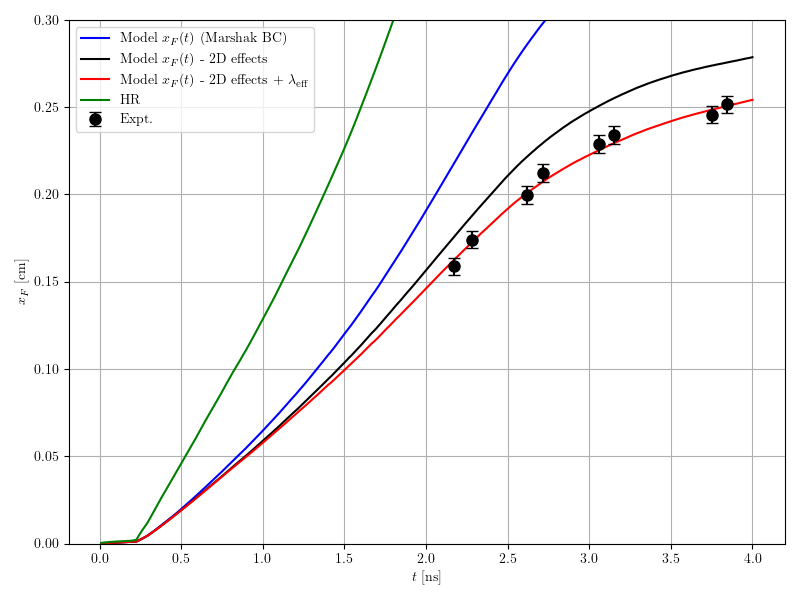
\includegraphics[width=0.49\columnwidth]{figures/C8H7Cl.png}
    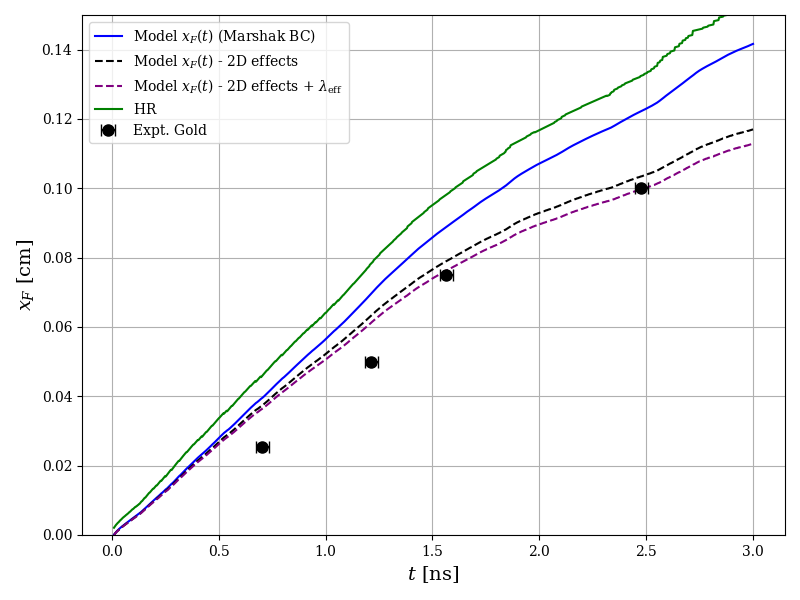
\includegraphics[width=0.49\columnwidth]{figures/Ta2O5.png}\\
    \vspace{0.1cm}
    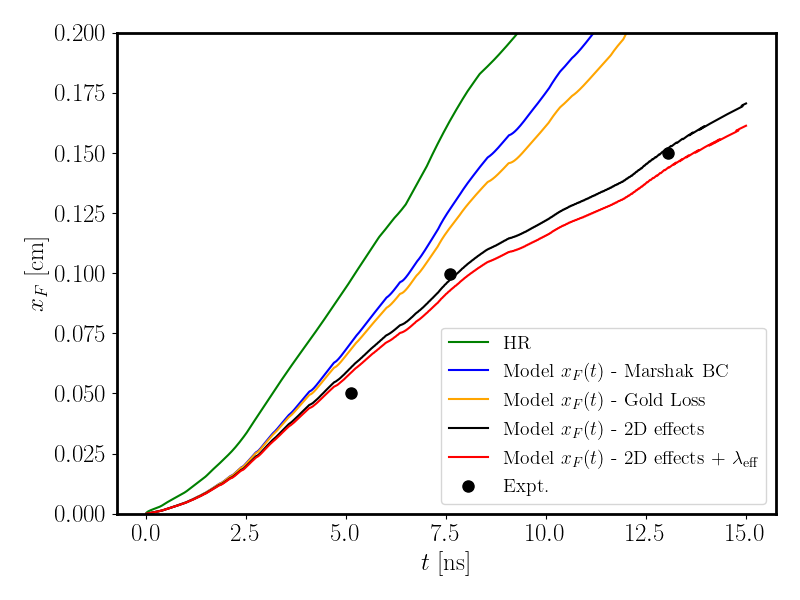
\includegraphics[width=0.49\columnwidth]{figures/SiO2_low_energy.png}
    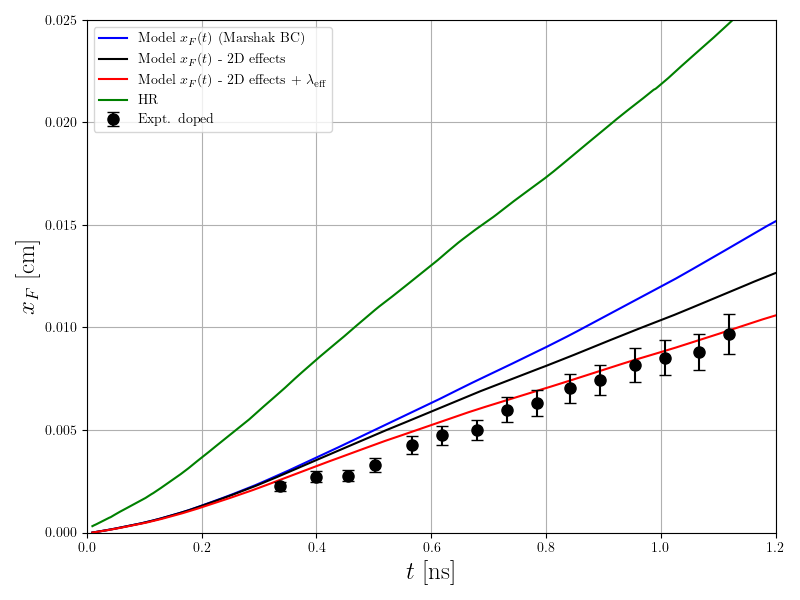
\includegraphics[width=0.49\columnwidth]{figures/Ji-Yan.png}
    \caption{Heat front position from the 1.5D model (solid curves) compared to experimental data (symbols) for four experiments:
    (a)~Moore \textit{et al.}~\cite{Moore2015}, $\mathrm{C}_8\mathrm{H}_7\mathrm{Cl}$;
    (b)~Back \textit{et al.}~\cite{Back2000POP}, $\mathrm{Ta}_2\mathrm{O}_5$;
    (c)~Back \textit{et al.}~\cite{Back2000PRL}, $\mathrm{SiO}_2$;
    (d)~Ji-Yan \textit{et al.}~\cite{JiYan2010}, $\mathrm{C}_8\mathrm{H}_8$.}
    \label{fig:1.5D_comparison}
\end{figure}

Figure~\ref{fig:1.5D_comparison} demonstrates that the 1.5D model, incorporating all four corrections, accurately reproduces the heat front position across four independent experiments spanning different foam materials (chlorinated polystyrene, tantala, silica, polystyrene), densities (10--160\,mg/cc), and drive temperatures (85--310\,eV).

% ============================================================================
%  IV. FULL 2D MODEL
% ============================================================================
\section{Full 2D Model}

\subsection{Radial curvature from the eigenvalue problem}

Hurricane and Hammer~\cite{Hurricane2006} showed that for constant opacity and negligible material energy, the diffusion equation reduces to Laplace's equation, whose solution in Cartesian slab geometry has a transverse cosine mode.
Courtois \textit{et al.}~\cite{Courtois2022} re-derived the solution in cylindrical coordinates, obtaining
\begin{equation}\label{eq:HH_cyl}
    x_F(r,t) = \frac{1}{\kappa_0}\cosh^{-1}\!\left(1 + \frac{D\kappa_0^2 t}{2}\right)J_0(\kappa_0 r) + \text{H.O.T.},
\end{equation}
where $J_0$ is the zeroth-order Bessel function and, for small $\varepsilon$,
\begin{equation}\label{eq:kappa0}
    \kappa_0 \approx \frac{\sqrt{2\varepsilon}}{R}, \quad \varepsilon = \tfrac{3}{4}\rho\kappa R(1 - a),
\end{equation}
with $a$ the wall albedo.
However, the longitudinal part of Eq.~(\ref{eq:HH_cyl}) is inaccurate because it neglects material energy storage and opacity temperature dependence.

\subsection{Dynamic albedo}

The wall albedo $a$ has previously been treated as a constant free parameter.
We compute it dynamically from the ratio of outgoing to incoming flux at the wall:
\begin{equation}\label{eq:albedo}
    \alpha(t) = \frac{\sigma_{\mathrm{SB}}T_{s,\mathrm{int}}^4 - \frac{1}{2}\frac{dE_{\mathrm{wall}}}{dt}}{\sigma_{\mathrm{SB}}T_{s,\mathrm{int}}^4 + \frac{1}{2}\frac{dE_{\mathrm{wall}}}{dt}},
\end{equation}
where $T_{s,\mathrm{int}}$ is the foam--wall interface temperature and $dE_{\mathrm{wall}}/dt$ is the wall energy absorption rate.
This yields a time-dependent $\varepsilon(t)$ and hence a time-dependent curvature.

\subsection{Combined 2D front}

The key insight is that the 1.5D model provides an accurate longitudinal front position $x_{\mathrm{1.5D}}(t)$, while the eigenvalue problem provides the correct radial shape.
We combine them as
\begin{equation}\label{eq:2D_front}
    \boxed{x_F(r,t) = x_{\mathrm{1.5D}}(t)\cdot J_0\!\left(\kappa_0(t)\,r\right).}
\end{equation}
The full temperature distribution is then obtained via the Henyey self-similar profile:
\begin{equation}\label{eq:T_profile}
    T(z,r,t) \approx T_S(t)\left[1 - \frac{z}{z_F(r,t)}\right]^{1/(4+\alpha-\beta)}.
\end{equation}

\begin{figure}[t]
    \centering
    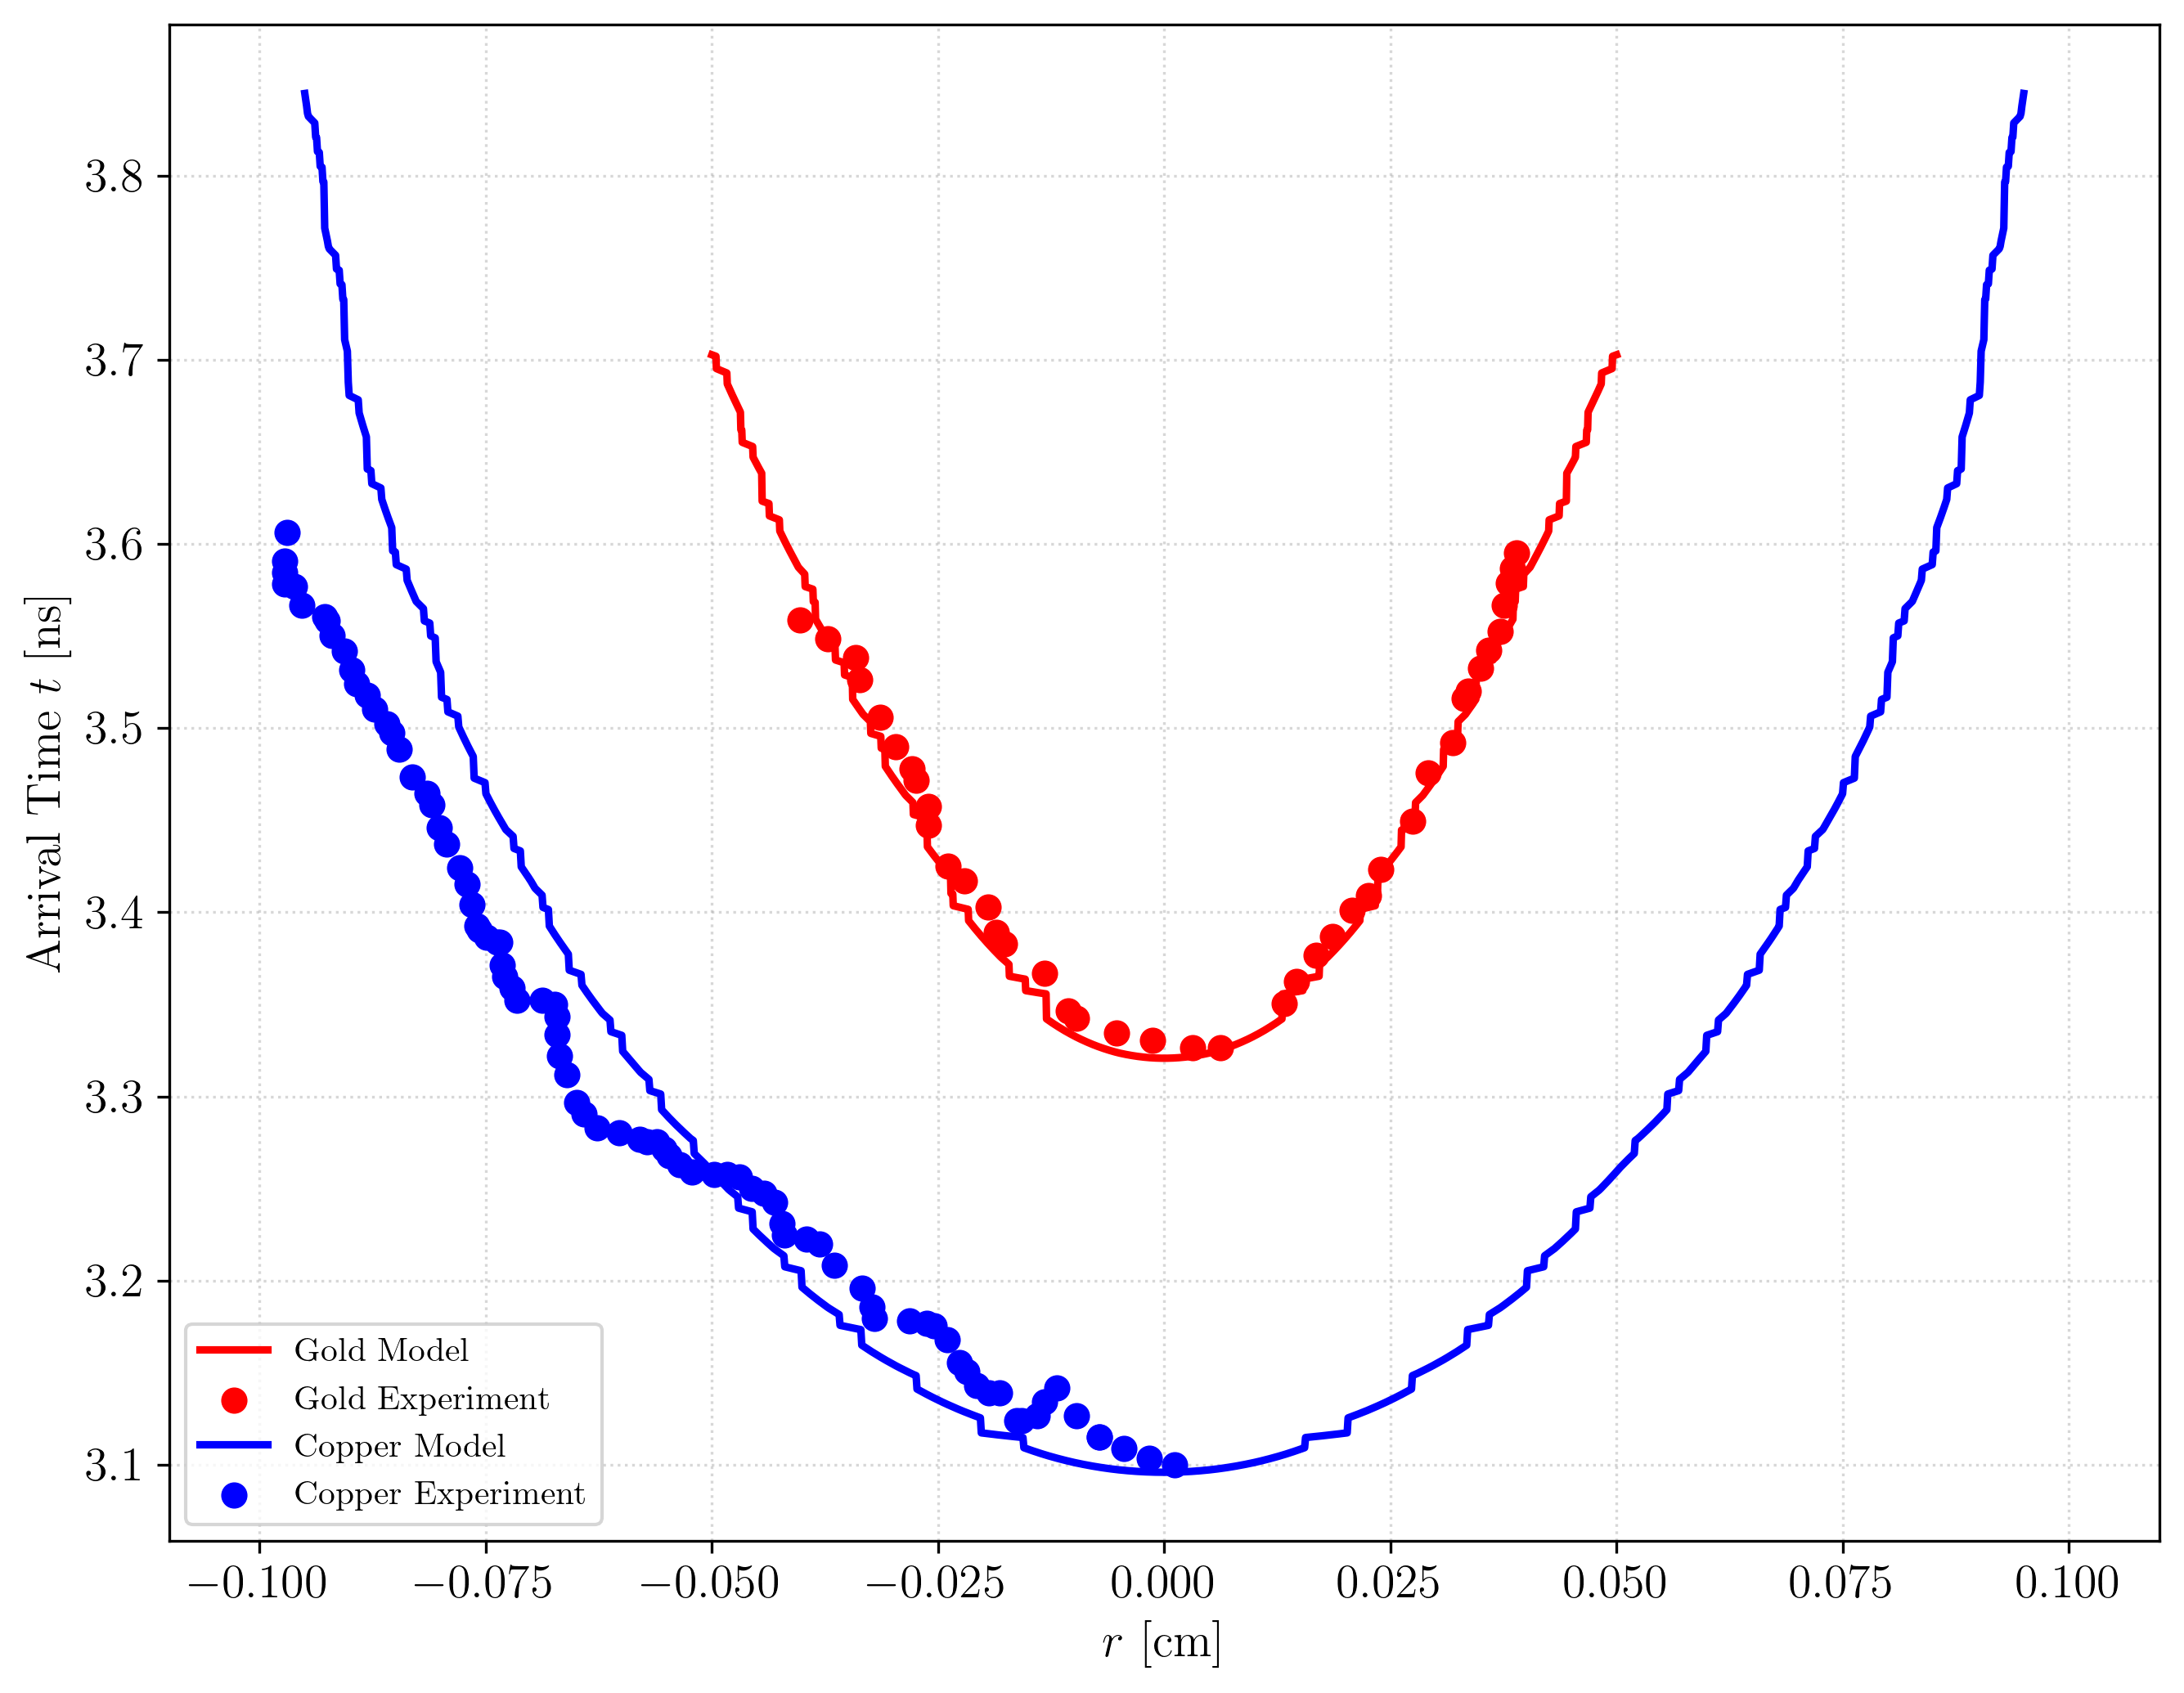
\includegraphics[width=\columnwidth]{figures/combined_curvature_comparison.png}
    \caption{Front arrival time as a function of radial position $r$ for gold-coated (left) and copper-coated (right) tubes, comparing the 2D model (solid curves) with the measurements of Courtois \textit{et al.}~\cite{Courtois2024}. The model captures the material-dependent curvature quantitatively.}
    \label{fig:curvature_comparison}
\end{figure}

\subsection{Validation}

We validate the 2D model against supersonic diffusion simulations for five wall materials (gold, gold$\times 100$ transparency, copper, beryllium, vacuum) with $\mathrm{SiO}_2$ foam.
In all cases, the model reproduces both the longitudinal front position and the radial curvature.

Figure~\ref{fig:curvature_comparison} shows a direct comparison with the experimental measurements of Courtois \textit{et al.}~\cite{Courtois2024}, who measured the front arrival time $t_F(r)$ for both gold and copper coatings.
The model correctly predicts the stronger curvature for gold (lower albedo, higher wall absorption) versus copper.

\begin{figure}[t]
    \centering
    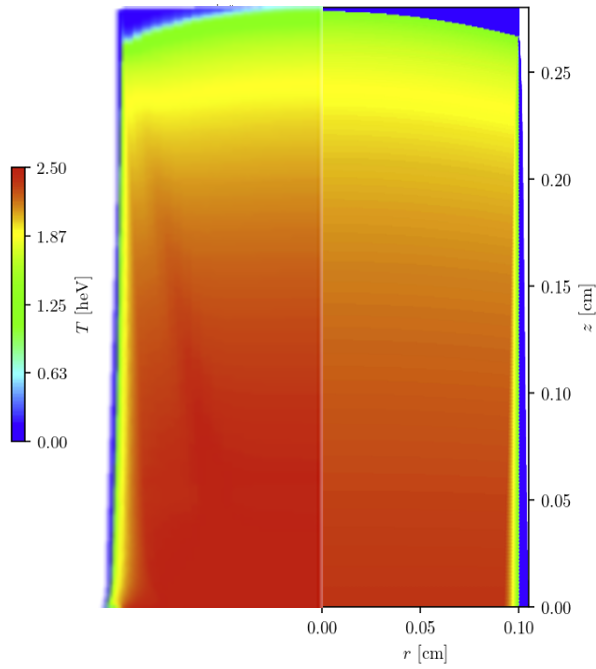
\includegraphics[width=\columnwidth]{figures/moore_simulation.png}
    \caption{2D temperature distribution for the Moore \textit{et al.}\ experiment ($\mathrm{C}_8\mathrm{H}_7\mathrm{Cl}$) at $t = 3.72$\,ns. Left: diffusion simulation from Ref.~\cite{Moore2015}. Right: present 2D model using Eqs.~(\ref{eq:2D_front})--(\ref{eq:T_profile}).}
    \label{fig:moore_2D}
\end{figure}

Figure~\ref{fig:moore_2D} compares the full 2D temperature distribution from our model with the 2D diffusion simulation of Moore \textit{et al.}~\cite{Moore2015} for chlorinated polystyrene foam at $t = 3.72$\,ns.
The front shape, curvature, and temperature gradient behind the front are in excellent agreement.

Further comparisons with IMC simulations of the Back \textit{et al.}\ experiment at $t = 1.0$, 2.0, and 2.5\,ns, and with the Ji-Yan \textit{et al.}\ experiment at $t = 0.5$, 1.0, and 1.3\,ns, confirm that the model accurately reproduces the evolving 2D temperature field across time.

\begin{figure}[t]
    \centering
    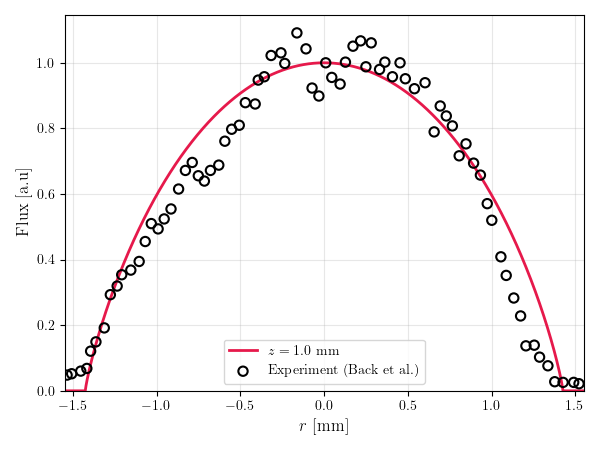
\includegraphics[width=\columnwidth]{figures/back_prl_curve.png}
    \caption{Spatial profile of the radiation flux emerging from the rear of a $\mathrm{SiO}_2$ foam sample. Symbols: experimental data from Back \textit{et al.}~\cite{Back2000PRL}. Curve: present 2D model. The agreement demonstrates that the model captures not only the front position but also the observable radiation field.}
    \label{fig:flux_curvature}
\end{figure}

As a particularly stringent test, Fig.~\ref{fig:flux_curvature} compares the predicted spatial profile of the emerging radiation flux with the measurements of Back \textit{et al.}~\cite{Back2000PRL}.
This observable probes both the radial curvature and the temperature distribution behind the front simultaneously.

% ============================================================================
%  V. CONCLUSION
% ============================================================================
\section{Conclusion}

We have developed a unified semi-analytic model for 2D supersonic Marshak waves in cylindrical geometry.
The 1.5D component systematically accounts for the Marshak boundary condition, wall energy loss, wall ablation with foam densification, and effective mean free path corrections.
The full 2D model combines this accurate longitudinal solution with a dynamically computed Bessel-function radial mode [Eq.~(\ref{eq:2D_front})].

The model reproduces the heat front position across seven experiments, matches 2D diffusion simulations for five wall materials, captures experimentally measured front curvatures for gold and copper coatings, and predicts the spatial profile of the emerging radiation flux.
By providing a physically transparent, computationally inexpensive alternative to full numerical simulations, this framework enables rapid exploration of the parameter space and deepens our understanding of radiation transport in confined geometries.

\begin{acknowledgments}
We thank the members of the HEDP group at the Hebrew University of Jerusalem for valuable discussions.
\end{acknowledgments}

% ============================================================================
%  REFERENCES
% ============================================================================
\begin{thebibliography}{99}

\bibitem{Marshak1958}
R.~E.~Marshak,
\textit{Effect of Radiation on Shock Wave Behavior},
Phys.\ Fluids \textbf{1}, 24 (1958).

\bibitem{Zel'dovich1967}
Ya.~B.~Zel'dovich and Yu.~P.~Raizer,
\textit{Physics of Shock Waves and High-Temperature Hydrodynamic Phenomena}
(Academic Press, New York, 1967).

\bibitem{Lindl2004}
J.~D.~Lindl, P.~Amendt, R.~L.~Berger \textit{et al.},
\textit{The physics basis for ignition using indirect-drive targets on the National Ignition Facility},
Phys.\ Plasmas \textbf{11}, 339 (2004).

\bibitem{Henyey1955}
L.~G.~Henyey,
unpublished (1955);
see also R.~E.~Marshak, Ref.~\cite{Marshak1958}, and
S.~Heizler and T.~Shussman,
Phys.\ Plasmas \textbf{22}, 082109 (2015).

\bibitem{Hammer2003}
J.~H.~Hammer and M.~D.~Rosen,
\textit{A consistent approach to solving the radiation diffusion equation},
Phys.\ Plasmas \textbf{10}, 1829 (2003).

\bibitem{Shussman2015}
T.~Shussman and S.~I.~Heizler,
\textit{Full self-similar solutions of the subsonic radiative heat equations},
Phys.\ Plasmas \textbf{22}, 082109 (2015).

\bibitem{Pomraning1979}
G.~C.~Pomraning,
\textit{The Equations of Radiation Hydrodynamics}
(Pergamon, Oxford, 1973).

\bibitem{Back2000PRL}
C.~A.~Back, J.~D.~Bauer, J.~H.~Hammer \textit{et al.},
\textit{Diffusive, supersonic x-ray transport in radiatively heated foam cylinders},
Phys.\ Rev.\ Lett.\ \textbf{84}, 274 (2000).

\bibitem{Back2000POP}
C.~A.~Back, J.~D.~Bauer, O.~L.~Landen \textit{et al.},
\textit{Detailed measurements of a diffusive supersonic wave in a radiatively heated foam},
Phys.\ Plasmas \textbf{7}, 2126 (2000).

\bibitem{Moore2015}
A.~S.~Moore, T.~M.~Guymer, J.~Morton \textit{et al.},
\textit{Characterization of supersonic radiation diffusion waves},
J.\ Quant.\ Spectrosc.\ Radiat.\ Transfer \textbf{159}, 100 (2015).

\bibitem{Hurricane2006}
O.~A.~Hurricane and J.~H.~Hammer,
\textit{Bent Marshak waves},
Phys.\ Plasmas \textbf{13}, 113303 (2006).

\bibitem{Courtois2022}
C.~Courtois, R.~Gr\"oger, P.~Loiseau \textit{et al.},
\textit{Models for the propagation of radiation heat fronts in cylindrical tubes},
Phys.\ Plasmas \textbf{29}, 022704 (2022).

\bibitem{Courtois2024}
C.~Courtois, R.~Gr\"oger, P.~Loiseau \textit{et al.},
\textit{Experimental measurements of supersonic radiation heat wave curvature in cylindrical tubes},
Phys.\ Plasmas \textbf{31}, 012707 (2024).

\bibitem{JiYan2010}
Z.~Ji-Yan, H.~Bo, Z.~Yong-Kuan \textit{et al.},
\textit{Simulation of 2D radiation transport in a cylindrical target},
Chin.\ Phys.\ B \textbf{19}, 025201 (2010).

\bibitem{Massen1994}
J.~Massen, G.~D.~Tsakiris, K.~Eidmann \textit{et al.},
\textit{Supersonic radiative heat waves in low-density foam targets},
Phys.\ Rev.\ E \textbf{50}, 5130 (1994).

\bibitem{Xu2010}
L.~Xu, Y.~Gu, Z.~Zheng \textit{et al.},
\textit{Observation of supersonic radiation diffusion wave in low-density plastic foam},
Eur.\ Phys.\ J.\ D \textbf{60}, 337 (2010).

\bibitem{Rosen2005}
M.~D.~Rosen, H.~A.~Scott, D.~E.~Hinkel \textit{et al.},
\textit{The role of a detailed configuration accounting (DCA) atomic physics package in explaining the energy balance in ignition-scale hohlraums},
High Energy Density Phys.\ \textbf{7}, 180 (2011).

\end{thebibliography}

\end{document}
